\documentclass[tikz,border=10pt]{standalone}
\usetikzlibrary{intersections}

\begin{document}
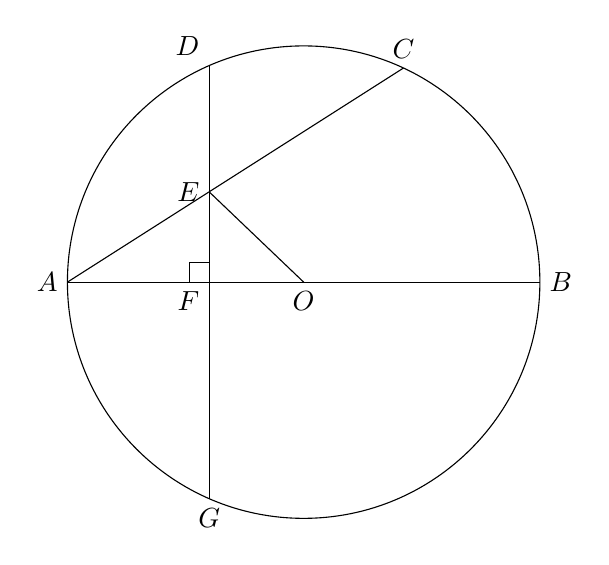
\begin{tikzpicture}
    % Define coordinates
    \coordinate (O) at (0,0);
    \coordinate (A) at (-3,0);
    \coordinate (B) at (3,0);
    
    % F is on AB. Let's place it at x = -1.2
    \coordinate (F) at (-1.2, 0);
    
    % D and G are on the circle, vertical line through F.
    % Radius is 3. y = sqrt(3^2 - 1.2^2) = sqrt(7.56) approx 2.75
    \coordinate (D) at (-1.2, 2.75);
    \coordinate (G) at (-1.2, -2.75);
    
    % C is on the circle. Angle 65 degrees to match visual proportions (E lower than midpoint)
    \coordinate (C) at (65:3);
    
    % Draw the circle
    \draw (O) circle (3);
    
    % Draw lines
    \draw (A) -- (B); % Diameter
    \draw[name path=chordDG] (D) -- (G); % Chord DG
    \draw[name path=chordAC] (A) -- (C); % Chord AC
    
    % Find intersection E
    \path [name intersections={of=chordAC and chordDG, by=E}];
    
    % Draw OE
    \draw (O) -- (E);
    
    % Right angle mark at F (Top-Left quadrant)
    \draw (F) ++(-0.25, 0) -- ++(0, 0.25) -- ++(0.25, 0);
    
    % Labels
    \node[left] at (A) {$A$};
    \node[right] at (B) {$B$};
    \node[above] at (C) {$C$};
    \node[above left] at (D) {$D$};
    \node[left] at (E) {$E$};
    \node[below left] at (F) {$F$};
    \node[below] at (G) {$G$};
    \node[below] at (O) {$O$};
    
\end{tikzpicture}
\end{document}
